\section*{Zielsetzung}
\label{sec:Zielsetzung}
In diesem Versuch soll mit dem photoelektrischen Effekt die Natur des Lichtes im Hinblick
auf einen Teilchencharakter untersucht werden.

\section{Theorie}
\label{sec:Theorie}

\subsection{Theoretische Betrachtung des Lichtes}
\label{sec:Theoretische Betrachtung des Lichtes}
Für die Deutung verschiedener Beobachtungen sind zwei verschiedene Theorien über die Natur
des Lichtes entstanden: Während für Versuche wie die Compton-Streuung oder die Paarbildung
das Licht als quantisierte, diskrete ``Energiepakete`` aufgefasst wird, können Phänomene
wir Beugung und Interferenz nur mit einem Wellencharakter erklärt werden.
Die beiden Modelle sind widersprüchlich; das folgt schon aus der mathematischen
Beschreibung. Während für Streuprozesse die Newtonsche (bzw. relativistische) Punktmechanik
verwendet wird, folgt die Wellenmechanik aus den Maxwellgleichung.
Eine widerspruchsfreie Theorie, die beide Fälle vereint, ist die Quantenelektrodynamik,
wobei dort Korpuskel- und Wellenmodell als Grenzfälle enthalten sind. Allgemein kann man
sagen, dass wenn eine große Anzahl Photonen betrachtet wird (zum Beispiel bei der
räumlichen Ausbreitung des Lichtes), die Wellentheorie ausreichend gute Ergebnisse
erzielt. Bei Interaktion mit Materie, wie bei Emission und Absorption, stellt die
Korpuskeltheorie eine gute Näherung dar. 

\subsection{Der Photoeffekt und die Erklärung im Kontext der Korpuskulartheorie}
\label{sec:Der Photoeffekt und die Erklärung im Kontext der Korpuskulartheorie}
Unter dem Photo- oder lichtelektrischen Effekt wird die Auslösung von Elektronen aus
Metall bei Bestrahlung mit Licht. Die erste qualitative Erklärung kam von Einstein im
Jahre 1905, diese beruhte auf der Korpuskulartheorie des Lichts, also der Betrachtung als
diskrete Objekte.
\\
Zur Untersuchung des Photoeffekts wird ein Aufbau wie in
\autoref{fig:PrinzipielleAnordnung} verwendet. In einem evakuiertem Aufbau wird eine als
Photokathode bezeichnete Metallfläche mit Licht bestrahlt und eine Auffängerelektrode
elektrisch positiv (im Bezug auf die Kathode) aufgeladen. Die Photoelektronen sind dann
als Strom zwischen den Elektroden messbar.
\begin{figure}
	\centering
	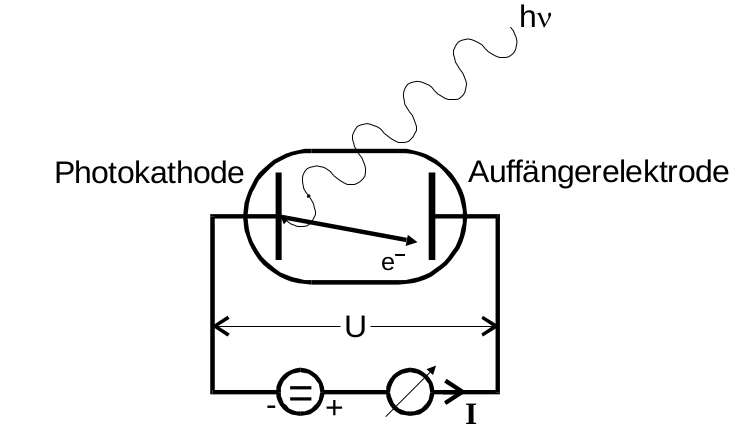
\includegraphics[height=5cm]{pictures/PrinzipielleAnordnung.png}
	\caption{Prinzipielle Anordnung zur Untersuchung des Photoeffektes}
	\label{fig:PrinzipielleAnordnung}
\end{figure}

